\documentclass{jhps}
\usepackage{amssymb}
\usepackage{mathtools}
\usepackage{booktabs}
\usepackage{multirow}
\usepackage{adjustbox}
\usepackage{footnote}
\usepackage{framed}
\usepackage{textcomp}
\usepackage{verbatim}
  %\usepackage{float}
  %\usepackage{array}
  %\usepackage{longtable}
\usepackage{adjustbox}
\usepackage{enumitem}
  %\usepackage{comment}
  %\usepackage{pdflscape}
  %\usepackage{adjustbox}
  %\usepackage{tabularx}

\graphicspath{
{./assets/}
}

\begin{document}

\JHPSissue{0}   % keep 0 until the issue is assigned
\JHPSkeywords{Compression, NetCDF}   % add 2-5 keywords

  % Author macro takes Name, Institution, Optional Link to the person, Optional Email
\JHPSauthor{Max Müller}{My institution\\Berlin, Germany}{https://myinstitution.com/max}{max@müller.com}
\JHPSauthor{Priya Singh}{Another affiliation\\Bangladesh, India}{}{}   % use empty email here

\title{My Title}

  % add the section numbers to the listings/figures/tables
\counterwithin{lstlisting}{section}
\counterwithin{figure}{section}
\counterwithin{table}{section}

\maketitle

\begin{abstract}
This is the abstract.
This is the abstract.
This is the abstract.
This is the abstract.
This is the abstract.
This is the abstract.
This is the abstract.
This is the abstract.
This is the abstract.
This is the abstract.
This is the abstract.
This is the abstract.
This is the abstract.
This is the abstract.
This is the abstract.
This is the abstract.
This is the abstract.
This is the abstract.
This is the abstract.
This is the abstract.
This is the abstract.
This is the abstract.
This is the abstract.
This is the abstract.
\end{abstract}

\section{Introduction}
\label{sec:intro}

This document describes the formatting for JHPS.
Please check the LaTeX source code.
In \Cref{sec:intro}, the formatting style for different elements is described.

\subsection{Tables}
  %\usepackage{tabu}
  %\taburulecolor{EsiOrange}

For tables with a header, please use the formatting in \Cref{tbl:1a}.
Provide the unit in a secondary row.
Tables without a header can use a closed box as in \Cref{tbl:1b}.

\begin{table}
  \centering
  \begin{subtable}[t]{8cm}
  \centering
  \begin{tabular}{l|l|l}
         \rowcolor{tblhead} Experiment  & Throughput & Total perf.
  \\
         \rowcolor{tblhead}   & in IOPS & in MiB/s \\
       \hline
       \hline
   Config 1 & 1   &  2   \\
  \hline
   Config 2 & 4   &  5   \\
  \end{tabular}
  \caption{Caption 1}\label{tbl:1a}
  \end{subtable}
  %%%
  \begin{subtable}[t]{3cm}
  \centering
  \begin{tabular}{|l|l|l|}
  \hline
   1   &  2   &  3  \\
  \hline
   4   &  5   &  6  \\
  \hline
  \end{tabular}
  \caption{Caption 2}\label{tbl:1b}
  \end{subtable}
  \caption{Main table caption}\label{tbl:1}
\end{table}

\subsection{Figures}

\begin{figure}   % don't change placement [bpt] if possible
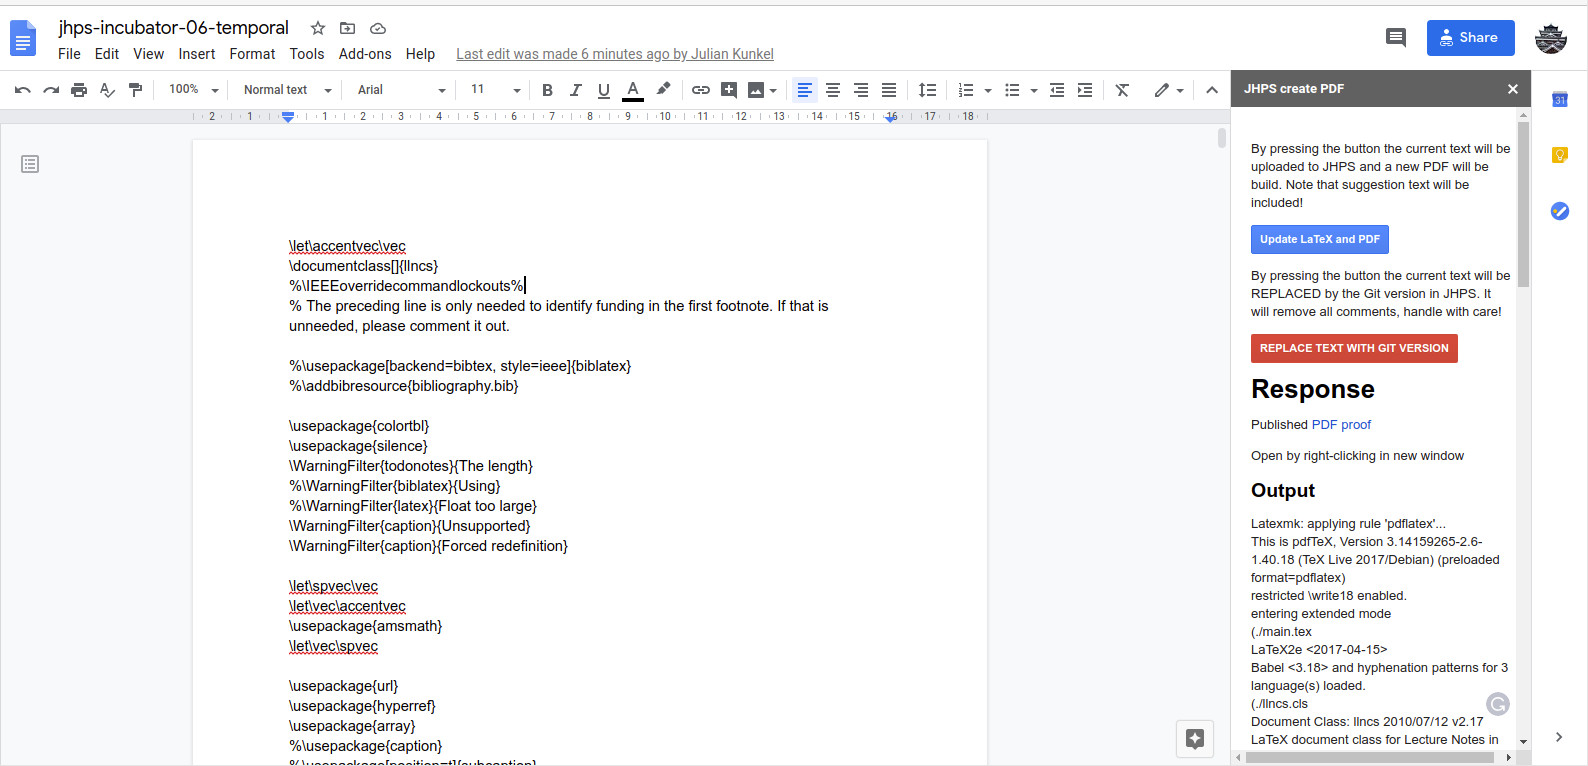
\includegraphics[width=0.8\textwidth]{jhps}
\caption{JHPS figure}
\label{fig:jhps}
\end{figure}

See \Cref{fig:jhps} for a simple figure.

\begin{figure}
  \begin{subfigure}[t]{3cm}
  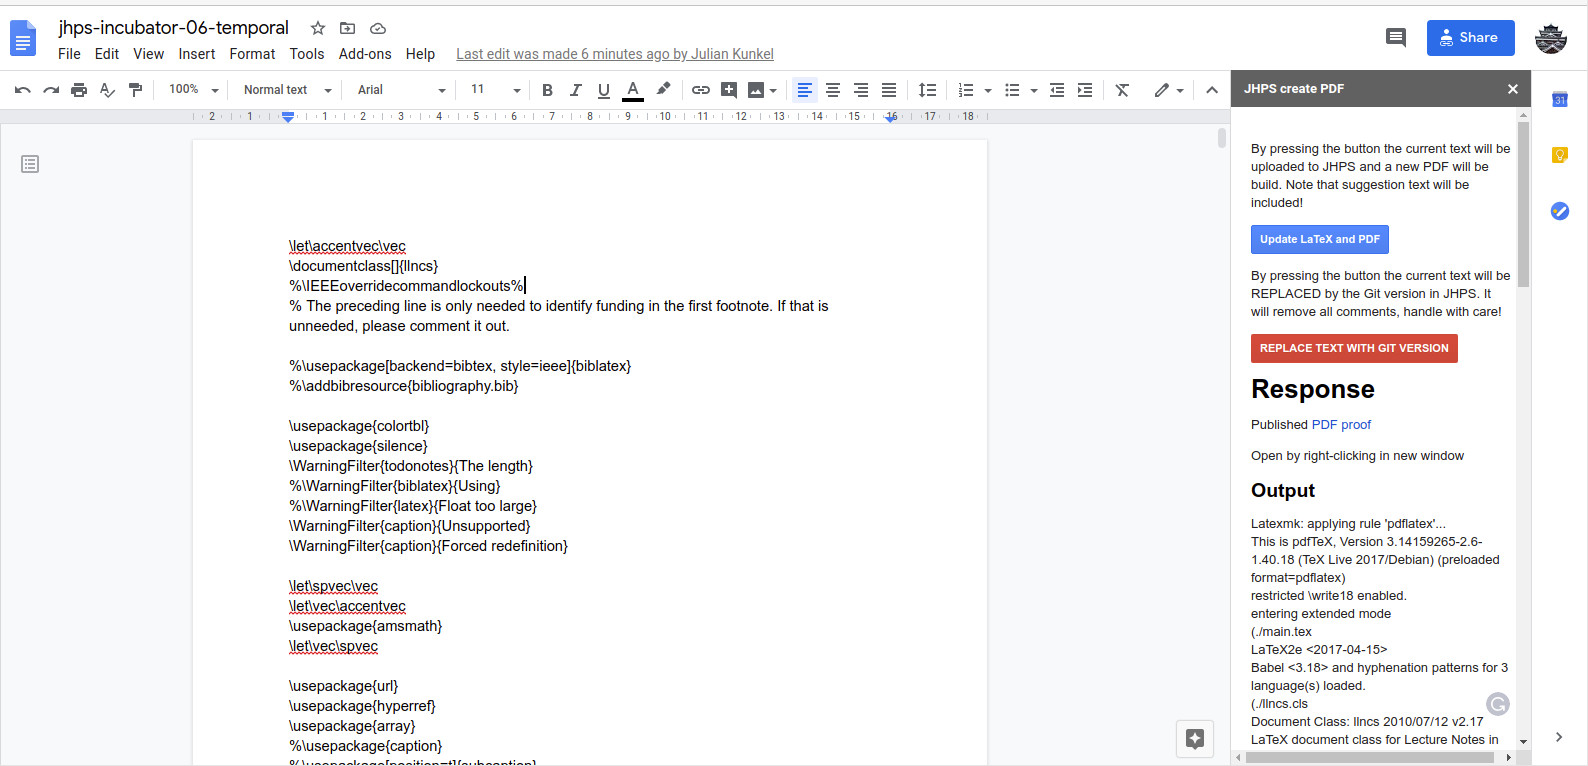
\includegraphics[width=\textwidth]{jhps}
  \caption{Caption 1}\label{fig:1a}
  \end{subfigure}
  \quad
  \begin{subfigure}[t]{3cm}
  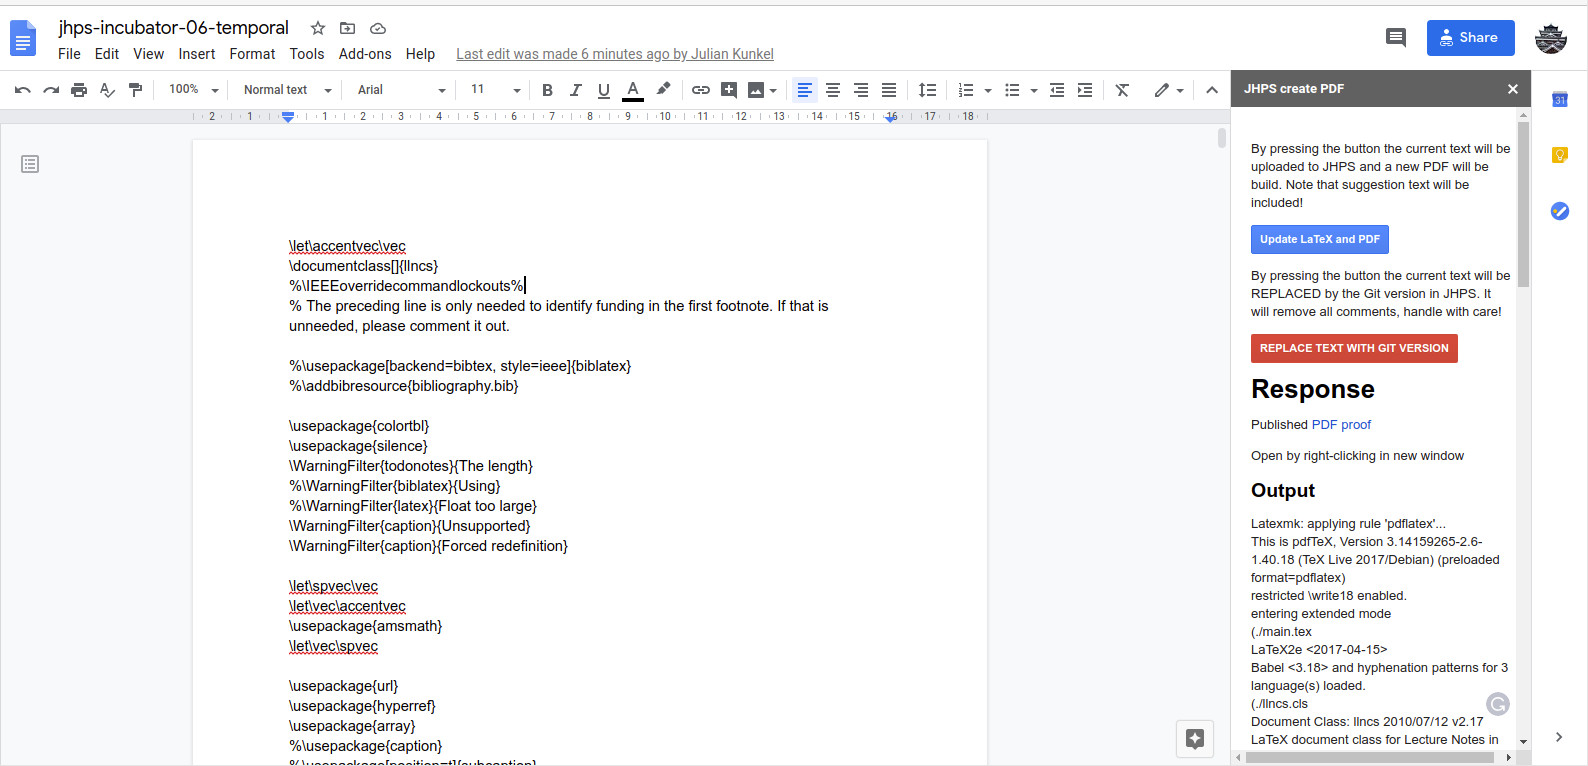
\includegraphics[width=\textwidth]{jhps}
  \caption{Caption 2}\label{fig:1b}
  \end{subfigure}
  \caption{Caption of the main figure}\label{fig:1}
\end{figure}

\subsection{Footnote}
Add\footnote{footnotes}.

\subsection{Links}
Generally, avoid using links in the text, but rather use a footnote, e.g.,
The webpage of JHPS\footnote{\url{https://jhps.vi4io.org}} provides author instructions.
You may also embed long links using HREF \href{https://jhps.vi4io.org}{JHPS Webpage}.

\subsection{Listings}

Use the lstlisting package for short inline listings here (ca.
5 lines) as in \Cref{lst:listing}.
Otherwise wrap it into the lstfloat environment as in \Cref{lst:longlisting}.

\begin{lstlisting}[caption="My listing",label=lst:listing,language=C]
int main(){
  int jhps = 1;
  printf("This article is in JHPS:   %d\n", jhps);
}
\end{lstlisting}

\begin{lstfloat}
  \begin{lstlisting}[caption="My longer listing",label=lst:longlisting,language=C]
int main(){
  // Comment
  /* comment */
  int jhps = 1;
  printf("This article is in JHPS:   %d\n", jhps);
}
  \end{lstlisting}
\end{lstfloat}

\subsection{Verbatim}
To create a verbatim environment, you can use:
\begin{verbatim}
\verb|Some verbatim text|
\end{verbatim}
or
\begin{verbatim}
\begin{verbatim}
Some verbatim text
\end{verbatim}
\vspace*{-0.8em}
\verb|\end{verbatim}|

\subsection{References}

Use the Cref command, e.g. \verb|\Cref{lst:listing}|.\subsection{Citations}

Please use the default style; example: \cite{misc1998}.
Please save the bibliography in the file \texttt{bibliography.bib}.

Generally, avoid using links in the bibliography, use a footnote instead.

\subsection*{Acknowledgment} %% Remove this section if not needed
\textit{We thank XX for sponsoring.}

  % The bibliography
\addcontentsline{toc}{section}{Bibliography}
\bibliography{bibliography.bib}

\reviews   % The review section

\subsection*{Reviewer: \href{Optional URL to reviewer page}{Firstname LastName}, Date: 2020-07-07}

\paragraph{Overall summary and proposal for acceptance}

\paragraph{Scope}   % in regards to the journal, i.e., does the topic fit?

\paragraph{Significance}   % of the research, minor vs. major

\paragraph{Readability}   % English and structure appropriate?

\paragraph{Presentation}

\paragraph{References}   % Correctly formatted?

\paragraph{Correctness}   % Is the research correct


\end{document}
